\documentclass{article}
\usepackage[utf8]{inputenc}

\usepackage{amsmath}
\usepackage{amssymb}
\usepackage{amsthm}
\usepackage{cancel}

\usepackage{caption}
\usepackage{graphicx}
\usepackage[top=0.5in, bottom=0.5in, left=1in, right=1in]{geometry}

\usepackage{titlesec}
    \titlespacing{\subsection}{\parindent}{15pt}{1pt}

\title{\textbf{\underline{CSCI3070U: Analysis and Design of Algorithms}\\Assignment 1}}
\author{Syed Arham Naqvi\\\\100590852}
\date{\today}

\begin{document}

    \maketitle

    \section*{Part 1.}
        \subsection*{a.}
            
            \begin{figure}[ht]
                
                \centering
                \begin{minipage}{0.9\textwidth}
                    
                    Given: $\mathbf{T(n) = 8T\left(\frac{n}{2}\right) + n log_{2}(n)}$.\\\\
                    $\mathbf{a} = 8$, $\mathbf{b} = 2$ and $\forall n > 1$, $\hspace{5pt} \mathbf{f(n)} = n \cdot \log_{2}(n) > 0$.\\\\
                    Note that for $c=1$ and $\forall n > n_{0} = 1$:
                    \begin{align*}
                                    f(n)    &= n \cdot \log_{2}(n)\\ 
                                            &\leq n^{2}\\
                                            &\leq n^{\log_{2}(8)}\\
                                            &= n^{3}
                    \end{align*}
                    So for $\epsilon = 1 > 0$ we can see that $f(n) = \mathcal{O}(n^{\log_{2}(8) - 1}) = \mathcal{O}(n^{3 - 1}) = \mathcal{O}(n^{2})$.\\\\
                    $\therefore \hspace*{5pt}$ by case 1 of the Master Theorem $T(n) = \Theta(n^{3})$ which implies $T(n) = \mathcal{O}(n^{3})$

                \end{minipage}

            \end{figure}
        
        \subsection*{b.}
            
            \begin{figure}[ht]
                \centering
                \begin{minipage}{0.9\textwidth}
                    Given: $\mathbf{T(n) = 7T\left(\frac{n}{2}\right)+n^{2}}$.\\\\
                    We can determine the upper bound of this recurrence using a recursion tree:\\
                \end{minipage}
                \begin{minipage}{0.9\textwidth}
                    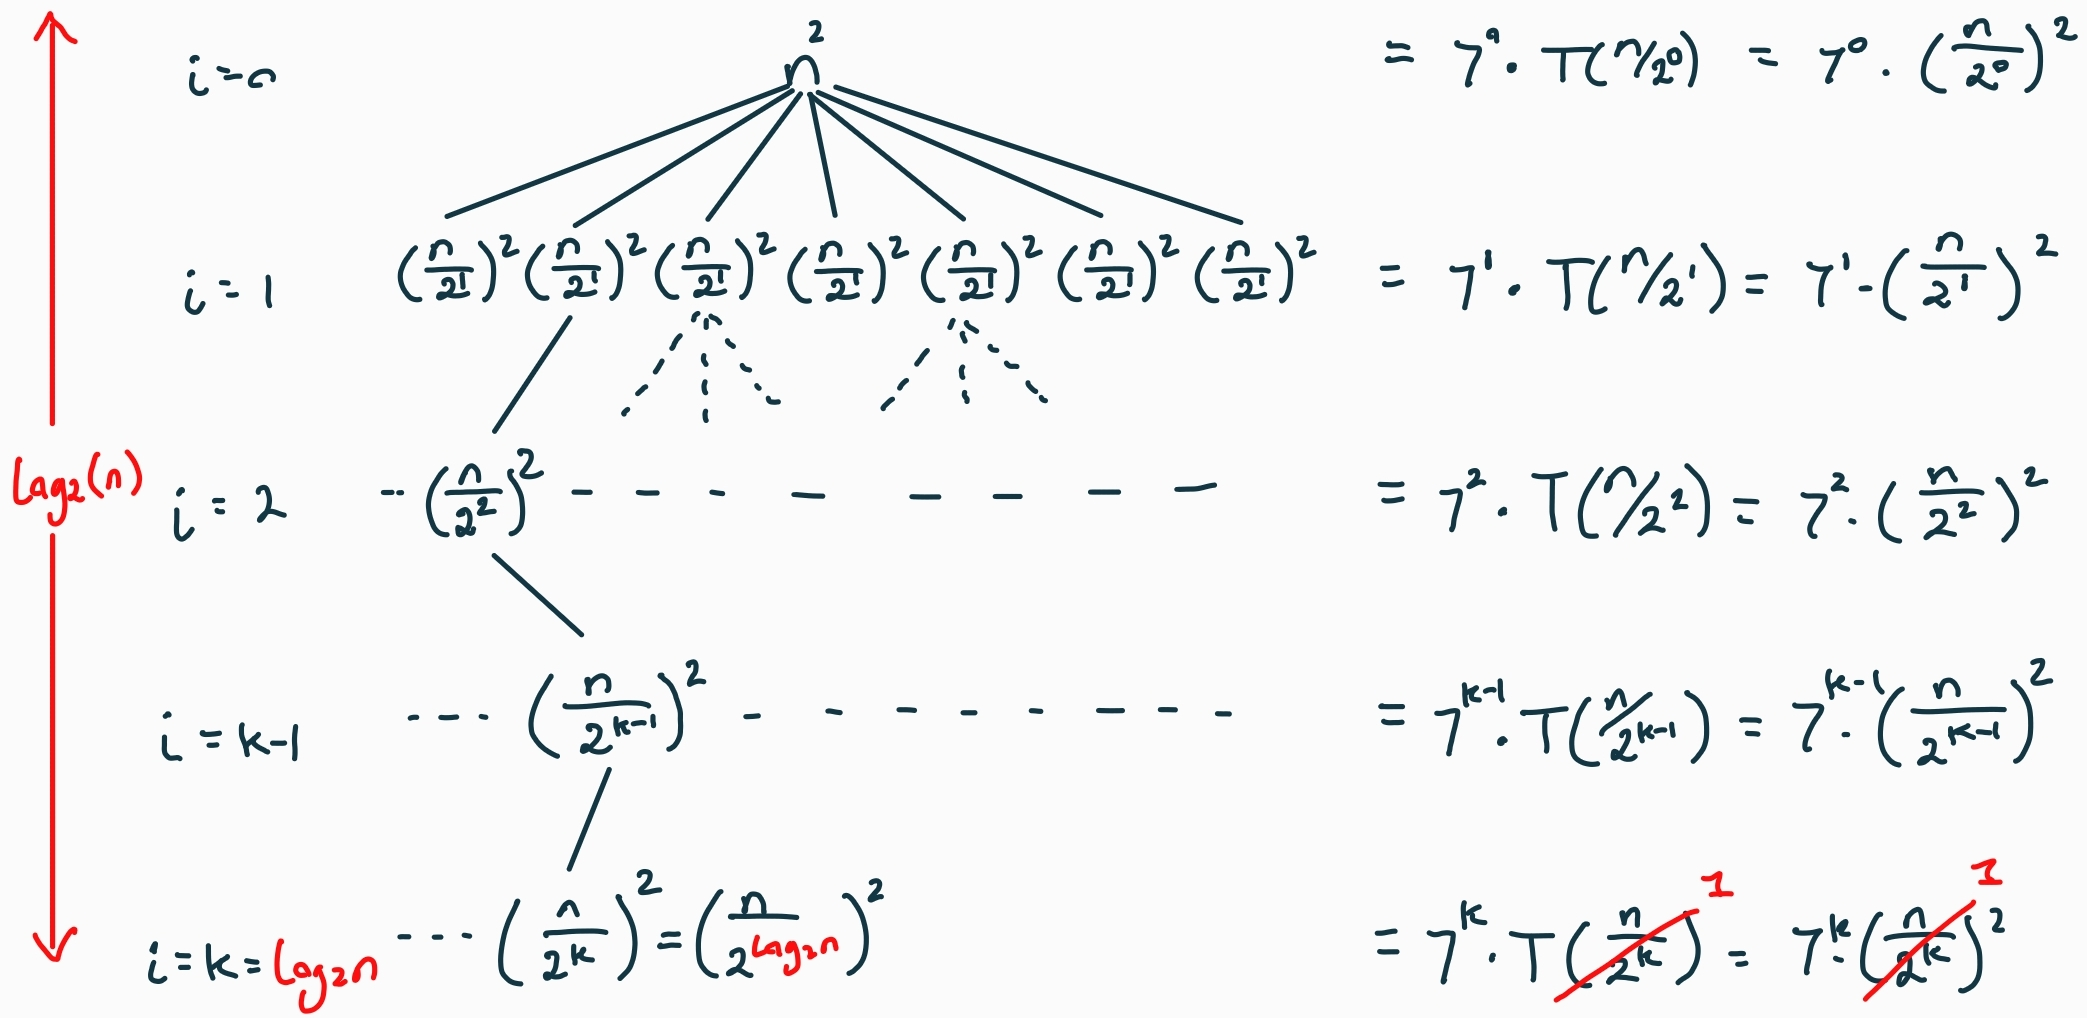
\includegraphics[width=5.3in]{1b_diagram.jpg}
                \end{minipage}
            \end{figure}

            \newpage

            \begin{figure}[!ht]
                \centering
                \begin{minipage}{0.9\textwidth}
                    We find that the complexity of a given recursion level ($i$), is represented by the expression:
                    
                    \begin{equation}                        
                        7^{i} \cdot \left(\frac{n}{2^{i}}\right)^{2}
                    \end{equation}
                    
                    Which can be simplified to:
                    
                    \begin{equation}
                        n^{2} \cdot \left(\frac{7}{4}\right)^{i}
                    \end{equation}

                    We now sum the cost of each level of recursion for $i \in [0,1\dots,k]$ where $k = \log_{2}(n)$:

                    \begin{align*}
                        T(n) &= \sum_{i=0}^{k} \left( n^{2} \cdot \left(\frac{7}{4}\right)^{i}\right)\\
                             &= n^{2} \cdot \sum_{i=0}^{k} \left(\frac{7}{4}\right)^{i}\\
                             &= n^{2} \cdot \left( \frac{\left(\frac{7}{4}\right)^{k+1} - 1} {\left(\frac{7}{4}\right) -1 } \right)\\
                             &= n^{2} \cdot \left( \frac{\left(\frac{7}{4}\right)^{\log_{2}(n)+1} - 1} {\left(\frac{3}{4}\right)} \right)\\
                             &= n^{2} \cdot \left( \frac{\left(\frac{7}{4}\right)^{\log_{2}(n)} \cdot \left(\frac{7}{4}\right) - 1} {\left(\frac{3}{4}\right)} \right)\\
                             &= n^{2} \cdot \left( \frac{n^{\log_{2}\left(\frac{7}{4}\right)} \cdot \left(\frac{7}{4}\right) - 1} {\left(\frac{3}{4}\right)} \right)\\
                             &= n^{2} \cdot \left( \frac{n^{\log_{2}(7)-\log_{2}(4)} \cdot \left(\frac{7}{4}\right) - 1} {\left(\frac{3}{4}\right)} \right)\\
                             &= n^{2} \cdot \left( \frac{n^{\log_{2}(7)-2} \cdot \left(\frac{7}{4}\right) - 1} {\left(\frac{3}{4}\right)} \right)\\
                             &= \frac{n^{\log_{2}(7)} \cdot \left(\frac{7}{4}\right) - n^{2}} {\left(\frac{3}{4}\right)}\\
                             &= \left(\frac{7}{3}\right)n^{\log_{2}(7)} - \left(\frac{4}{3}\right)n^{2} \\
                             &\leq c \cdot n^{\log_{2}(7)} \hspace*{5pt} \text{for}
                             \hspace*{5pt} c = 3 \hspace*{5pt} \text{and} \hspace*{5pt} \forall n > n_{0} = 1
                    \end{align*}

                    $\therefore \hspace*{5pt}$ we have demonstrated using a recursion tree that $T(n) = \mathcal{O}(n^{log_{2}(7)})$.

                \end{minipage}
            \end{figure}
        
        \newpage

        \subsection*{c.}

            \begin{figure}[!ht]
                
                \centering
                \begin{minipage}{0.9\textwidth}
                    \textbf{Given:} $\mathbf{T(n) = T\left(\frac{n}{2}\right) + T\left(\frac{n}{4}\right) + T\left(\frac{n}{8}\right) + 1}$.\\
                    \textbf{Guess:} $T(n)$ is $\mathcal{O}(\log_{2}(n))$.\\
                    
                    For the inductive process, we will assume that $n_{0} = 2$ and that $T(n_{0}) = T(2) = 2$ for our inductive base case.\\
                    
                    \textbf{Induction:}\\
                    \hspace*{10pt} Basis: For $n_{0} = 2$, $T(2) = 2 \leq c \cdot \log_{2}(2)$, $\forall c \geq 2$.\\
                    \hspace*{10pt} Inductive step: Inductive hypothesis is that $\forall k < n$, $T(k) \leq c \cdot \log_{2}(k)$ where $c \geq 2$.
                    \begin{align*}
                        T(n) &= T\left(\frac{n}{2}\right) + T\left(\frac{n}{4}\right) + T\left(\frac{n}{8}\right) + 1\\
                             &\leq c_{1} \cdot \log_{2}\left(\frac{n}{2}\right) + c_{2} \cdot \log_{2}\left(\frac{n}{4}\right) + c_{3} \cdot \log_{2}\left(\frac{n}{8}\right) + 1\\
                             &= c_{1} \cdot (\log_{2}n - \log_{2}2) + c_{2} \cdot (\log_{2}n - \log_{2}4) + c_{3} \cdot (\log_{2}n - \log_{2}8) + 1\\
                             &= c_{1} \cdot (\log_{2}n - 1) + c_{2} \cdot (\log_{2}n - 2) + c_{3} \cdot (\log_{2}n - 3) + 1\\
                             &\leq c_{1} \cdot (\log_{2}n) + c_{2} \cdot (\log_{2}n) + c_{3} \cdot (\log_{2}n) + c_{4} \cdot (\log_{2}n)\\
                             &= \underbrace{(c_{1} + c_{2} + c_{3} + c_{4})}_{c} \cdot (\log_{2}n)\\
                             &= c \cdot \log_{2}n
                    \end{align*}

                    $\therefore \hspace*{5pt}$ we have shown using the substitution method and the inductive process that $T(n) = \mathcal{O}(\log_{2}n)$.
                \end{minipage}

            \end{figure}
        
        \subsection*{d.}

            \begin{figure}[!ht]
                
                \centering
                \begin{minipage}{0.9\textwidth}
                    Given: $\mathbf{T(n) = \sqrt{200} \cdot T\left(\frac{n}{2}\right) + n^{\sqrt{200}}}$.\\

                    $\mathbf{a} = \sqrt{200}$, $\mathbf{b} = 2$ and 
                    $ \forall n > 0$,  $\mathbf{f(n)} = n^{\sqrt{200}} > 0$.\\

                    If we can find some $t > 0$ such that $f(n) = n^{\log_{b}a + t}$, then we can find some $\epsilon$ where $0 < \epsilon < t$ so that $f(n) > n^{\log_{b}a + \epsilon}$:
                    \begin{align*}
                        f(n)            &=  n^{\log_{b}(a) + t}\\
                        n^{\sqrt{200}}  &=  n^{\log_{2}(\sqrt{200}) + t}\\
                        10\sqrt{2}      &=  \log_{2}(10\sqrt{2}) + t\\
                        t               &=  10\sqrt{2} - \log_{2}(10\sqrt{2})\\
                        t               &\approx 10.32
                    \end{align*}
                    Let $\epsilon = 5$ so that $0 < \epsilon < t$ and $n^{\sqrt{200}} > n^{\log_{2}(\sqrt{200}) + 5}$ which means $f(n) = \Omega({n^{\log_{b}(a) + \epsilon}})$.\\
                    We now verify the regularity condition:
                    \begin{align*}
                        af\left(\frac{n}{2}\right)                                                               &\leq  cf(n)\\
                        \sqrt{200}\left(\frac{n}{2}\right)^{\sqrt{200}}                                          &\leq  cn^{\sqrt{200}}\\
                        \frac{(\sqrt{200})\cancel{(n^{\sqrt{200}})}}{\cancel{(n^{\sqrt{200}})}(2^{\sqrt{200}})}  &\leq  c\\
                        7.83 \cdot 10^{-4}                                                                       &\leq  c
                    \end{align*}
                    Thus if we let $c = \frac{1}{2}$, the regulaity condition holds.\\\\
                    $\therefore \hspace*{5pt}$ by case 3 of the master theorem, $T(n) = \Theta(n^{\sqrt{200}})$ which implies that $T(n) = \mathcal{O}(n^{\sqrt{200}})$.
                \end{minipage}

            \end{figure}
    
    \newpage

    \section*{Part 2.}
        
        \subsection*{a.}

            \begin{figure}[!ht]

                \centering
                \begin{minipage}{0.9\textwidth}
                    \textbf{Proposition:} For all positive $f(n)$, $g(n)$ and $h(n)$, if $f(n) = \mathcal{O}(g(n))$ and $h(n) = \Omega(f(n))$
                    then $g(n) + h(n) = \Omega(f(n))$.\\

                    This proposition is \textbf{true}.\\

                    If $f(n) = \mathcal{O}(g(n))$ then $\exists c, n_{0} > 0 \hspace*{3pt} | \hspace*{3pt} \forall n \geq n_{0}, \hspace*{3pt} f(n) \leq c \cdot g(n)$.\\
                    Let $k = \frac{1}{c}$ so $k > 0$ since $c > 0$.\\
                    It follows that $k \cdot f(n) \leq g(n)$ meaning that $g(n) = \Omega(f(n))$.\\
                    
                    If $h(n) = \Omega(f(n))$ then $\exists t, p_{0} > 0 \hspace*{3pt} | \hspace*{3pt} \forall n \geq p_{0}, \hspace*{3pt} t \cdot f(n) \leq h(n)$.\\

                    Now,
                    \begin{align*}
                        t \cdot f(n) + k \cdot f(n)                  &\leq          h(n) + g(n) \hspace{25pt}\text{ since } f(n), g(n), h(n), k, t > 0\\
                        \underbrace{(t + k)}_{r} \cdot f(n)          &\leq          h(n) + g(n)\\
                        r \cdot f(n)                                 &\leq          h(n) + g(n) \hspace{25pt}\text{ where } r > 0\\
                        h(n) + g(n)                                  &=             \Omega(f(n))\\
                    \end{align*}
                    $\therefore$ if $f(n) = \mathcal{O}(g(n))$ and $h(n) = \Omega(f(n))$ then $g(n) + h(n) = \Omega(f(n))$.
                \end{minipage}

            \end{figure}
    
        \subsection*{b.}

            \begin{figure}[!ht]

                \centering
                \begin{minipage}{0.9\textwidth}
                    \textbf{Proposition:} If $f(n) = \mathcal{O}(g(n))$ and $g(n) = \mathcal{O}(f(n))$ then $f(n) = g(n))$.\\
                    
                    This proposition is \textbf{false}.\\

                    Let $f(n) = n^{2} + n$ and $g(n) = n^{2}$ so $f(n) \neq g(n)$.\\
                    Take $k = 1$ and $n_{0} = 1$, then $\forall n \geq n_{0}, \hspace{3pt} g(n) \leq k \cdot f(n)$
                    meaning $g(n) = \mathcal{O}(f(n))$.\\
                    Now consider,
                    \begin{align*}
                        f(n)                                                            &\leq   c \cdot g(n)\\
                        n^{2} + n                                                       &\leq   c \cdot n^{2}\\
                        1 + \frac{1}{n}                                                 &\leq   c \hspace*{50pt} \text{since} \hspace*{3pt} n > 0\\
                        \lim_{n \to \infty} \left(1 + \cancelto{0}{\frac{1}{n}}\right)  &\leq   \lim_{n \to \infty} (c)\\
                        1                                                               &\leq   c
                    \end{align*}
                    If we let $c = 2$ then,
                    \begin{align*}
                        n^{2} + n                                                       &=      2 \cdot n^{2}\\
                        1 + \frac{1}{n}                                                 &=      2\\
                        n                                                               &=      1
                    \end{align*}
                    so $\forall n > n_{0} = 1$ and for $c = 2$, $f(n) \leq c \cdot g(n)$ which means $f(n) = \mathcal{O}(g(n))$.\\

                    $\therefore$ we have shown it to be possible that $g(n) = \mathcal{O}(f(n))$ and $f(n) = \mathcal{O}(g(n))$ and yet $f(n)\neq (g(n))$.
                \end{minipage}

            \end{figure}

\end{document}